\lecture{1. Introduction}{01}
% - Exactly two or three sections (other than the summary).
% - At *most* three subsections per section.
% - Talk about 30s to 2min per frame. So there should be between about
%   15 and 30 frames, all told.

\section{Introduction}

\begin{frame}
\frametitle{Is God a Divine Watchmaker?}
\begin{center}
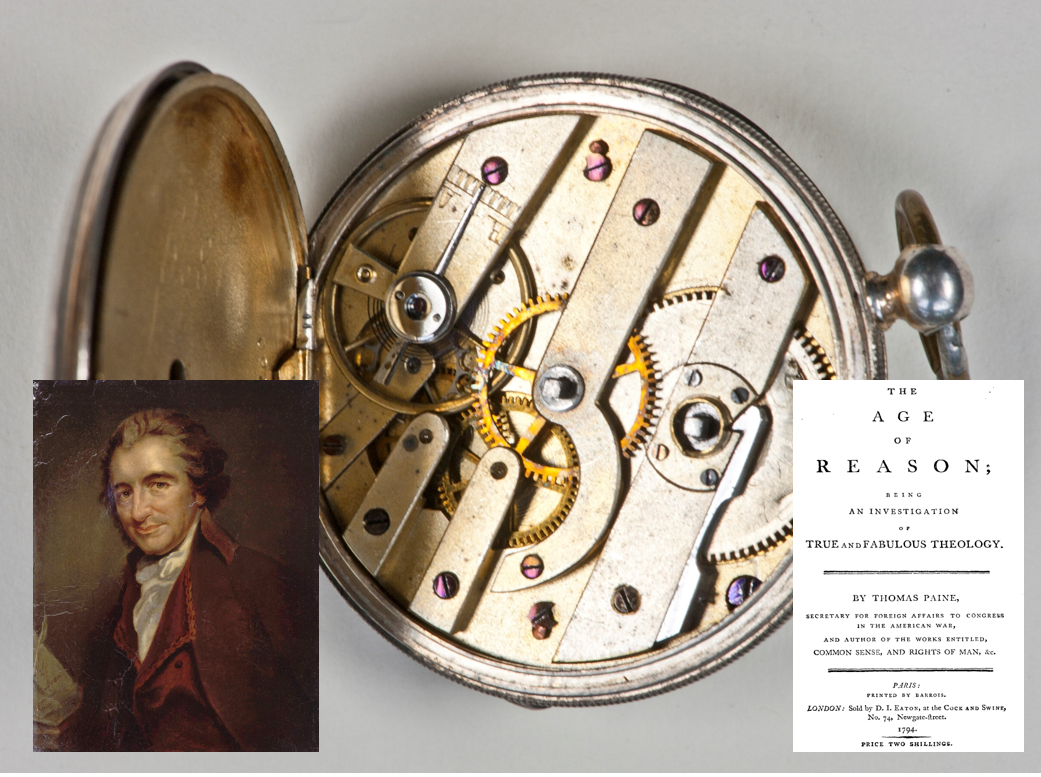
\includegraphics[width=0.92\textwidth]{figures/deism.png}
\end{center}
\end{frame}

%\begin{goals}
%\goal Become familiar with the class theme, key passage, and class objectives.
%\goal Understand how each subsequent lesson fits into the class objectives.
%\goal Do an initial evaluation of how relationship-focused your religion is.
%\end{goals}

\section{Class Overview}
\begin{frame}
\frametitle{Theme}
\begin{center}
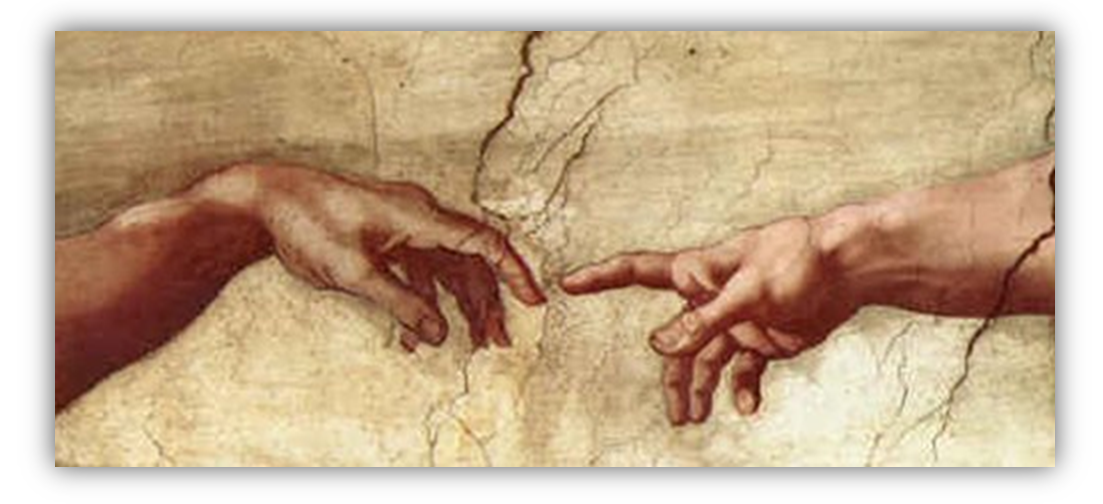
\includegraphics[width=0.7\textwidth]{figures/creation_of_adam.png}\\\vspace{1em}
\Large God wants a relationship with people.

\end{center}
\end{frame}

\begin{frame}
\frametitle{Key Passage}
\framesubtitle{Jeremiah 31:31-34}
\keyverse
\end{frame}

\begin{frame}
\frametitle{What makes Jer. 31:31-34 special?}
\framesubtitle{It describes what will change from the old covenant to the new.}
\begin{columns}
\begin{column}{0.4\textwidth}
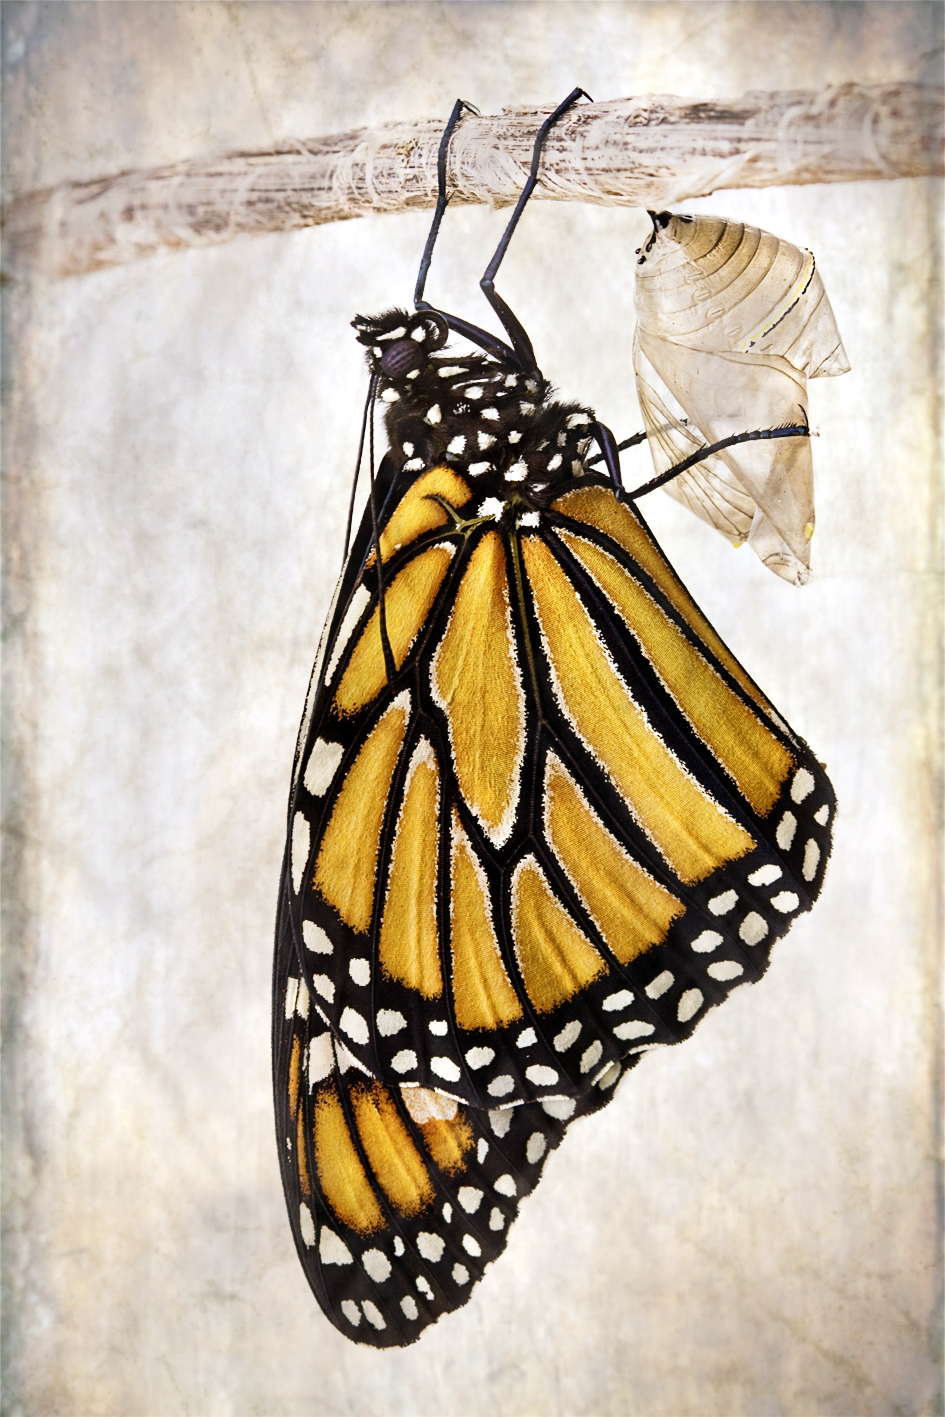
\includegraphics[width=\columnwidth]{figures/metamorphosis.jpg}
\end{column}
\begin{column}{0.6\textwidth}
\begin{itemize}
\item It is the only Old Testament verse with the term `new covenant'.
\item It contrasts old covenant faults with new covenant benefits.\\{\footnotesize (Heb. 8:1-13)}
\item It has the repeated Bible phrase, ``I will be their God and they shall be my people.'', which emphasizes relationship.\\{\footnotesize (Ex. 6:1-9, Lev. 22:31-33, etc.)}
\item It connects forgiveness of sins to our relationship with God.\\ {\footnotesize(John 3:16)}
\end{itemize}
\end{column}
\end{columns}
\end{frame}

\begin{frame}
\frametitle{Class Objectives}
	\begin{columns}
	\begin{column}{0.4\textwidth}
		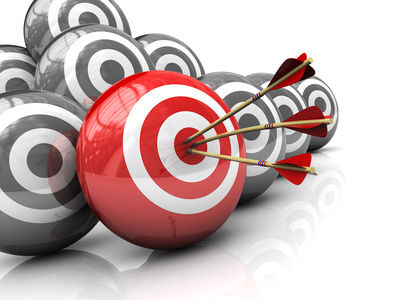
\includegraphics[width=\columnwidth]{figures/objectives.jpg}
	\end{column}
	\begin{column}{0.6\textwidth}
		\begin{itemize}
		\item Know the big picture of the Bible:\\\emph{God wants a relationship with a holy people who voluntarily choose Him}
		\item Understand how the relationship between God and His people grew from the Old Covenant to the New Covenant.
		\item Develop a relationship perspective in your own walk with God.
		\end{itemize}
	\end{column}
	\end{columns}
\end{frame}

\section{Lesson Overview}

\begin{frame}
\frametitle{Using your workbook}
\begin{columns}
\begin{column}{0.4\textwidth}
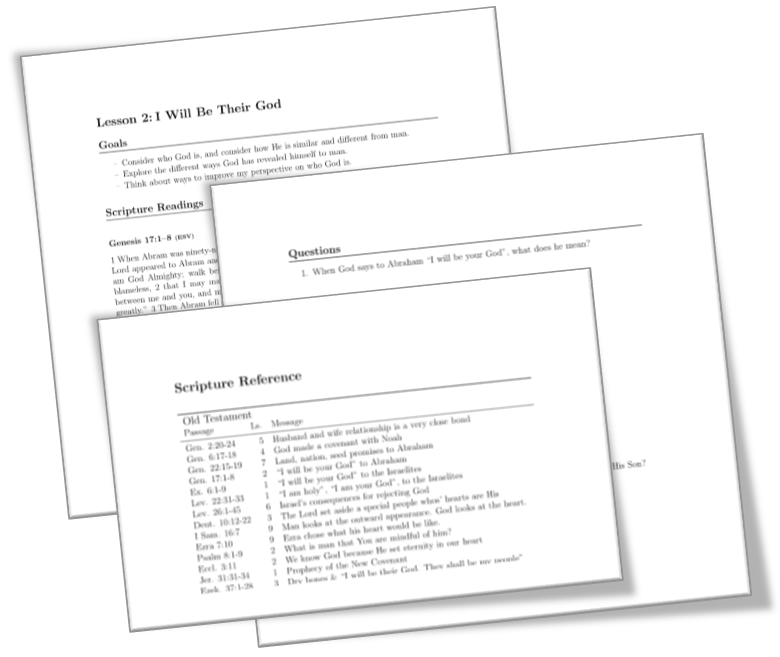
\includegraphics[width=1.3\columnwidth]{figures/workbook.PNG}
\end{column}
\begin{column}{0.6\textwidth}
\begin{itemize}
\item Each lesson begins with some goals for what we want to get out of the class.
\item All the scriptures necessary for the study are provided. \alert{Read these if nothing else}
\item There are four questions with each lesson that can be answered from the scriptures readings.
\item The ``Scripture Reference'' page is provided to help you remember the message of the passages we'll be reading.
\end{itemize}
\end{column}
\end{columns}
\end{frame}

\begin{frame}
\frametitle{Lessons}
\begin{columns}[T]
\begin{column}{0.5\textwidth}
\begin{enumerate}
\setcounter{enumi}{1}
\item  I Will Be Their God 
\item  They Shall Be My People 
\item  The Covenant I Made With Their Fathers 
\item  I Was Their Husband 
\item  My Covenant They Broke 
\item  Behold The Days Are Coming 
\end{enumerate}
\end{column}
\begin{column}{0.5\textwidth}
\begin{enumerate}
\setcounter{enumi}{7}
\item  I Will Make A New Covenant 

\item  Written On Their Hearts 

\item  For They Shall All Know Me 

\item  From The Least To The Greatest 

\item  I Will Forgive Their Iniquity 

\item  Review 
\end{enumerate}
\end{column}
\end{columns}
\end{frame}

\section{Review}

%\begin{frame}
%\frametitle{A first cut at the 'relationship' God}
	%\begin{description}[Lev. 22:31-33]
	%\item[Heb. 8:1-13] The Old Covenant had faults and is replaced with the New
	%\item[Ex. 6:1-9] ``I will be your God'' to the Israelites
	%\item[Lev. 22:31-33] ``I am holy'', ``I am your God'', to the Israelites
	%\item[John 3:16] God's love is His motivation for our salvation
	%\end{description}
%\end{frame}

\begin{frame}
\frametitle{Questions to ask yourself}
\framesubtitle{There's a difference between thinking and knowing}
\begin{columns}
	\begin{column}{0.3\textwidth}
		
\includegraphics[width=\columnwidth]{figures/contemplating.png}
	\end{column}
	\begin{column}{0.7\textwidth}
		\begin{itemize}	
		\item Is a relationship really what God is looking for from me?
		\item Is a relationship really what I'm looking for from God?
		\item What can I do to grow my relationship with God?
		\item How will I know that I'm closer to God?
		\end{itemize}
	\end{column}
\end{columns}
\end{frame}

%\begin{discussion}
%\dsubsec{Introduction}{900-905}{5}
%
%This lesson is about who God is.
%
%\bvs{Genesis}{(17:1-8)} God's first covenant with Abraham says that he will be his God.
%
%\dsubsec{Who is God?}{905-915}{10}
%
	%\bvs{Psalms}{(8:1-9)} It's amazing that God is is mindful of us.
%
%\dsubsec{How we come to know about God}{915-925}{10}
%
	%\bvs{Ecclesiastes}{(3:11)} Eternity in the heart of man
%
  %\bvs{Hebrews}{(1:1-2)} Fathers by the prophets, today His son
	%
	%By extension His Word.
%
%\dsubsec{What does that mean for me?}{925-940}{15}
%
	%\bvs{Luke}{(4:1-13)} Having a God gives you an anchor. 
	%
	%\bvs{Luke}{(14:25-27)} Love God and you will live.
%
%\dsubsec{Review}{940-945}{5}
%\end{discussion}

%\begin{frame}{Class Theme}{Subtitles are optional.}
  %% - A title should summarize the slide in an understandable fashion
  %%   for anyone how does not follow everything on the slide itself.
%
  %\begin{itemize}
  %\item
    %Use \texttt{itemize} a lot.
  %\item
    %Use very short sentences or short phrases.
  %\end{itemize}
%\end{frame}
%\begin{frame}{Lesson Motivation}{Subtitles are optional.}
  %% - A title should summarize the slide in an understandable fashion
  %%   for anyone how does not follow everything on the slide itself.
%
  %\begin{itemize}
  %\item
    %Use \texttt{itemize} a lot.
  %\item
    %Use very short sentences or short phrases.
  %\end{itemize}
%\end{frame}
%\begin{frame}{Lesson Objectives}{Subtitles are optional.}
  %% - A title should summarize the slide in an understandable fashion
  %%   for anyone how does not follow everything on the slide itself.
%
  %\begin{itemize}
  %\item
    %Use \texttt{itemize} a lot.
  %\item
    %Use very short sentences or short phrases.
  %\end{itemize}
%\end{frame}
%\section{Point1}
%\section{Point2}
%\section{Point3}
%\subsection[Objectives]{Theme}
%\subsection[Short First Subsection Name]{First Subsection Name}
%
%\begin{frame}{Make Titles Informative. Use Uppercase Letters.}{Subtitles are optional.}
  %% - A title should summarize the slide in an understandable fashion
  %%   for anyone how does not follow everything on the slide itself.
%
  %\begin{itemize}
  %\item
    %Use \texttt{itemize} a lot.
  %\item
    %Use very short sentences or short phrases.
  %\end{itemize}
%\end{frame}
%
%\begin{frame}{Make Titles Informative.}
%
  %You can create overlays\dots
  %\begin{itemize}
  %\item using the \texttt{pause} command:
    %\begin{itemize}
    %\item
      %First item.
      %\pause
    %\item    
      %Second item.
    %\end{itemize}
  %\item
    %using overlay specifications:
    %\begin{itemize}
    %\item<3->
      %First item.
    %\item<4->
      %Second item.
    %\end{itemize}
  %\item
    %using the general \texttt{uncover} command:
    %\begin{itemize}
      %\uncover<5->{\item
        %First item.}
      %\uncover<6->{\item
        %Second item.}
    %\end{itemize}
  %\end{itemize}
%\end{frame}
%
%
%\subsection{Second Subsection}
%
%\begin{frame}{Make Titles Informative.}
%\end{frame}
%
%\begin{frame}{Make Titles Informative.}
%\end{frame}
%
%
%
%\section*{Summary}
%
%\begin{frame}{Summary}
%
  %% Keep the summary *very short*.
  %\begin{itemize}
  %\item
    %The \alert{first main message} of your talk in one or two lines.
  %\item
    %The \alert{second main message} of your talk in one or two lines.
  %\item
    %Perhaps a \alert{third message}, but not more than that.
  %\end{itemize}
  %
  %% The following outlook is optional.
  %\vskip0pt plus.5fill
  %\begin{itemize}
  %\item
    %Outlook
    %\begin{itemize}
    %\item
      %Something you haven't solved.
    %\item
      %Something else you haven't solved.
    %\end{itemize}
  %\end{itemize}
%\end{frame}
